\subsection*{Основные формулы}

Коэффициент ослабления:
\begin{equation}
    \mu = \frac{1}{l} \ln \frac{N_0}{N},
    \label{base}
\end{equation}
где $l$ -- толщина образца, $N_0$ -- число падающих частиц и $N$ -- число частиц прошедших через образец.

Ниже, на рисунке \ref{fig:3}, приведена зависимость полного коэффициента ослабления потока $\gamma$-лучей для алюминия, железа и свинца, по которой можно восстановить энергию $\gamma$-квантов.


\begin{figure}[h]
    \centering
    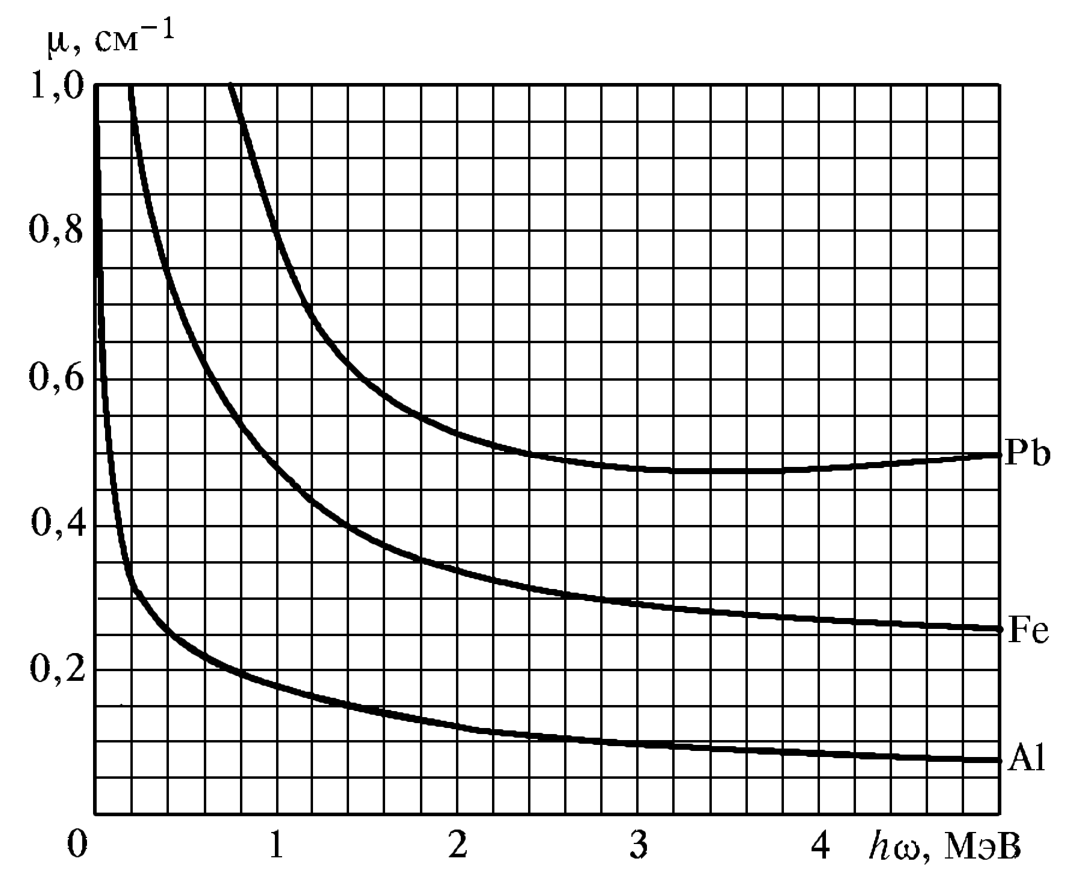
\includegraphics[width=0.4\textwidth]{figures/plot_lab.png}
    \caption{Полные коэффициенты ослабления потока $\gamma$-лучей в алюминии, железе и свинце.}
    \label{fig:3}
\end{figure}
